\section{El caso de los 100.000 correos}\label{sec:comparacion:caso}

Una aplicación necesita enviar 100.000 correos al mes, con ráfagas de 1.000 peticiones por minuto (16,7 peticiones por segundo), \textit{webhooks} de eventos y envío en lote.
¿Qué API y qué plan lo cubren al menor coste?
Parece que basta con buscar en cada página de precios el plan de 100.000 correos.
Pero la ráfaga se mide en peticiones y la cuota en correos, y una petición de lote lleva muchos correos.
¿Cuenta como un correo un mensaje con varios destinatarios, o como tantos como destinatarios lleve?
¿Y rigen los mismos límites si la aplicación envía por el relé SMTP y no por la API REST?

Es el ejemplo de la Sección~\ref{subsec:introduccion:ejemplo}.
Las cuatro condiciones se comprueban sobre la API REST, la interfaz que modelan las Datasheets (Sección~\ref{sec:propuesta:seleccion}).
El relé SMTP, la otra interfaz del canal API, queda fuera de la comparación.

Tres de las cuatro condiciones se leen en la Datasheet de cada API, y la cuarta fuera de ella.
El volumen sale de la cuota del plan y de su sobrecoste, y el coste se calcula para un mes de 30 días sumando al precio del plan el sobrecoste de los correos que pasan de la cuota.
La ráfaga se compara con el \textit{rate} del \textit{endpoint} de envío que recoge el campo \texttt{max\_power}, el caudal máximo que admite el plan.
El lote es el tope de destinatarios o mensajes por petición (el máximo del \texttt{workload}) del \textit{endpoint} que envía varios mensajes por llamada, y el caso no fija su tamaño.
Los \textit{webhooks} no son un campo de ACM2YAML v0.3, y se leen en la matriz de \textit{features} de cada API, fuera de la Datasheet.\footnote{\texttt{03\_datos/apis/<api>/features.md} del repositorio del trabajo, fila de \textit{webhooks} de eventos, con la fuente de cada celda.}

De cada API se toma el plan más barato que cubre los 100.000 correos y se comprueban en él las otras tres condiciones.
La Tabla~\ref{tab:comparacion:caso} recoge el resultado.

\begin{table}[tbp]
\centering
\small
\begin{tabular}{|p{2.0cm}|p{3.2cm}|p{2.2cm}|p{1.9cm}|p{2.0cm}|p{1.5cm}|}
\hline
\textbf{API} & \textbf{Plan y coste al mes (USD)} & \textbf{\textit{Rate} de envío} & \textbf{Lote} & \textbf{\textit{Webhooks}} & \textbf{Cumple} \\
\hline
SendGrid & Essentials 50K con sobrecoste: 19,95 + 50.000 $\times$ 0,0013 = 84,95 & 10.000 pet./s \semverde{} & 1.000 destinatarios & 2 \textit{endpoints} incluidos & sí \\
\hline
Mailgun & Scale: 90 con 100.000 incluidos & 1.500 pet./s \semambar{} & 1.000 destinatarios & en todos los planes & sí \\
\hline
Postmark & Platform con sobrecoste: 18 + 90.000 $\times$ 0,0012 = 126 & 5.000 pet./s \semambar{} & 500 mensajes & solo Pro y Platform & sí \\
\hline
Brevo & Professional: 499 con 150.000 incluidos & 1.000 pet./s \semambar{} & 2.000 destinatarios \semambar{} & en todos los planes & sí \\
\hline
Resend & Pro con sobrecoste: 20 + 50.000 $\times$ 0,0009 = 65 & 10 pet./s \semverde{} & 100 mensajes & 5 \textit{endpoints} en Pro & no \\
\hline
MailerSend & Starter con sobrecoste: 35 + 50.000 $\times$ 0,0013 = 100 & 120 pet./min \semverde{} & 35.000 destinatarios & 50 \textit{endpoints} en Starter & no \\
\hline
Amazon SES & sin cuota incluida, y el precio por destinatario no es campo & no publicado \semrojo{} & sin tope publicado & no (vía SNS) & no \\
\hline
Mailchimp Transactional & 4 bloques $\times$ 20 \semambar{} = 80, más una cuenta de Mailchimp de pago & no publicado \semrojo{} & sin tope publicado & por la API, en la cuenta de pago & sin respuesta \\
\hline
\end{tabular}
\caption[Respuesta del catálogo al caso de los 100.000 correos]{Plan más barato que cubre 100.000 correos al mes en cada API y comprobación de las otras tres condiciones: ráfaga de 1.000 peticiones por minuto, envío en lote y \textit{webhooks} de eventos. Coste con los campos \texttt{price}, \texttt{value} y \texttt{overage\_cost}. En Mailgun se toma \texttt{rate\_request\_api}, el caudal que aplica el motor. El del \textit{endpoint} de envío, 80.000 peticiones por ventana, también cumple la ráfaga: se midió en un sondeo, con una ventana de 9,85 a 9,87 segundos que la Datasheet redondea a 10, y está en ámbar. Los \textit{webhooks} se dan para el plan de la fila. El lote se da en destinatarios o en mensajes, según cuente cada proveedor. El \textit{rate} de Postmark se mide en la cabecera \texttt{ratelimit-limit} de un sondeo y no está publicado. Semáforo de la Datasheet: \semverde{} valor respaldado por su fuente, \semambar{} interpretado, \semrojo{} no publicado.}
\label{tab:comparacion:caso}
\end{table}

Con los campos de las Datasheets y la matriz de \textit{features} cumplen cuatro APIs: SendGrid, Mailgun, Postmark y Brevo.
Leyendo solo los campos, la más barata es SendGrid Essentials 50K con 50.000 correos de sobrecoste, a 84,95 USD, seguida de SendGrid Pro, a 89,95 USD con 100.000 correos incluidos, y de Mailgun Scale, a 90 USD.
En Postmark el plan más barato para este volumen es Platform, a 126 USD, porque su sobrecoste por correo es el menor de los tres planes de pago (Pro saldría a 133,50 USD).
Brevo exige Professional, a 499 USD, porque su Datasheet modela Starter y Standard con 5.000 correos y sin sobrecoste.
El tope de sobrecoste de SendGrid, diez veces el volumen del plan, no se alcanza con 100.000 correos (P-07, el tope que v0.3 no recoge, Sección~\ref{subsec:evolucion:p07}).

Si solo se leen los campos, Resend cubre el volumen por menos dinero que ninguna otra, 65 USD, y MailerSend lo cubre por 100 USD, pero las dos fallan en la ráfaga.
Resend admite 10 peticiones por segundo por equipo, 600 por minuto, en todos sus planes.
MailerSend admite 120 peticiones por minuto en \texttt{/v1/email} y 15 en \texttt{/v1/bulk-email} con el plan Starter.
El requisito cuenta peticiones y no correos: leído como 1.000 correos por minuto, las dos lo cumplirían enviando en lote.
La Figura~\ref{fig:comparacion:caso} sigue el caso en MailerSend Starter y muestra en qué unidad cuenta cada paso.

\begin{figure}[tbp]
\centering
\begingroup\hyphenpenalty=10000\relax
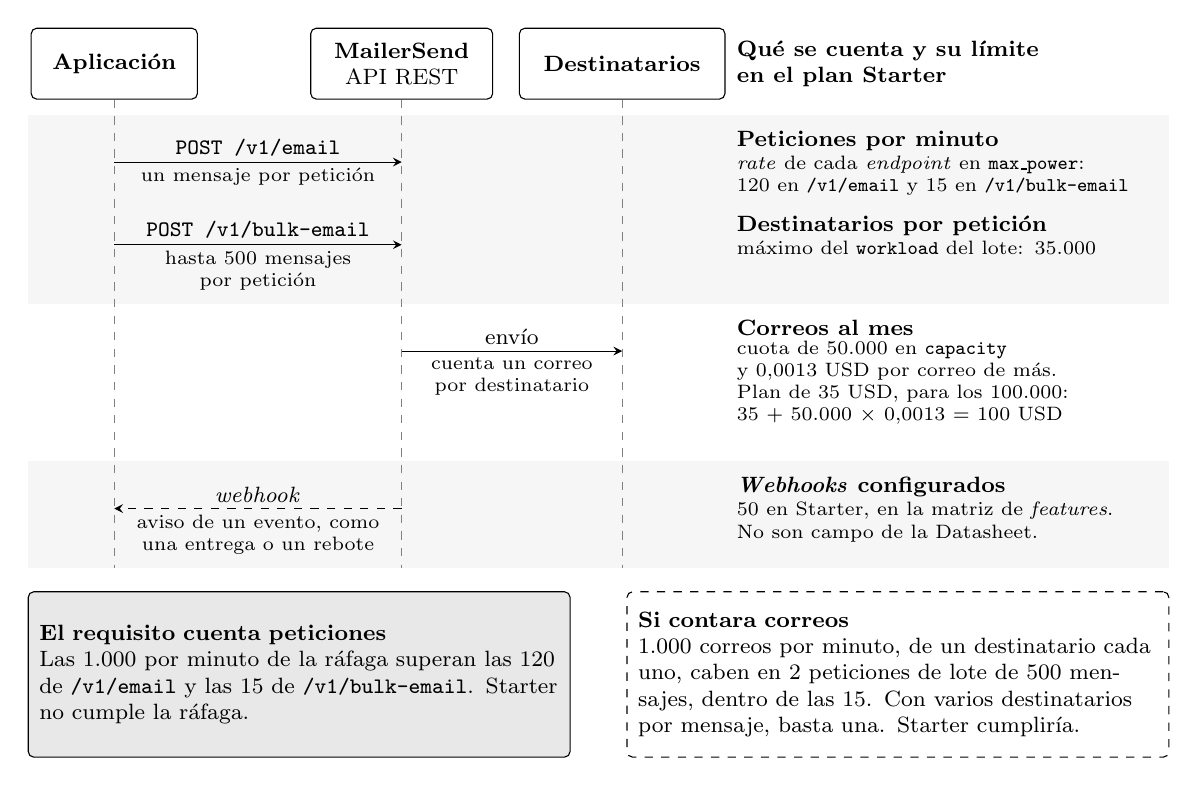
\begin{tikzpicture}[
  font=\footnotesize,
  actor/.style={draw, rounded corners=2pt, align=center, minimum height=9mm, inner sep=3pt},
  cabecera/.style={font=\footnotesize\bfseries, align=left, anchor=west, inner sep=0pt},
  arriba/.style={font=\footnotesize, anchor=south, inner sep=2pt},
  abajo/.style={font=\scriptsize, align=center, anchor=north, inner sep=2pt},
  unidad/.style={font=\footnotesize\bfseries, align=left, text width=55mm, anchor=north west, inner sep=0pt},
  limite/.style={font=\scriptsize, align=left, text width=55mm, anchor=north west, inner xsep=0pt, inner ysep=1.5pt},
  lectura/.style={draw, rounded corners=2pt, align=left, text width=66mm, minimum height=21mm, inner sep=4pt}
]
\fill[gray!7] (0,-1.15) rectangle (14.5,-3.55);
\fill[gray!7] (0,-5.55) rectangle (14.5,-6.9);
\node[actor, text width=19mm] (app) at (1.1,-0.5) {\textbf{Aplicación}};
\node[actor, text width=21mm] (api) at (4.75,-0.5) {\textbf{MailerSend}\\ API REST};
\node[actor, text width=24mm] (dest) at (7.55,-0.5) {\textbf{Destinatarios}};
\node[cabecera, text width=55mm] at (9.0,-0.5) {Qué se cuenta y su límite\\ en el plan Starter};
\draw[dashed, gray] (app.south) -- (1.1,-6.9);
\draw[dashed, gray] (api.south) -- (4.75,-6.9);
\draw[dashed, gray] (dest.south) -- (7.55,-6.9);
\draw[-stealth] (1.1,-1.75) -- node[arriba] {\texttt{POST /v1/email}} node[abajo] {un mensaje por petición} (4.75,-1.75);
\draw[-stealth] (1.1,-2.8) -- node[arriba] {\texttt{POST /v1/bulk-email}} node[abajo] {hasta 500 mensajes\\ por petición} (4.75,-2.8);
\node[unidad] (u1) at (9.0,-1.35) {Peticiones por minuto};
\node[limite] (l1) at (u1.south west) {\textit{rate} de cada \textit{endpoint} en \texttt{max\_power}:\\ 120 en \texttt{/v1/email} y 15 en \texttt{/v1/bulk-email}};
\node[unidad] (u2) at ([yshift=-2mm]l1.south west) {Destinatarios por petición};
\node[limite] at (u2.south west) {máximo del \texttt{workload} del lote: 35.000};
\draw[-stealth] (4.75,-4.15) -- node[arriba] {envío} node[abajo] {cuenta un correo\\ por destinatario} (7.55,-4.15);
\node[unidad] (u3) at (9.0,-3.75) {Correos al mes};
\node[limite] at (u3.south west) {cuota de 50.000 en \texttt{capacity}\\ y 0,0013 USD por correo de más.\\ Plan de 35 USD, para los 100.000:\\ 35 + 50.000 $\times$ 0,0013 = 100 USD};
\draw[-stealth, dashed] (4.75,-6.15) -- node[arriba] {\textit{webhook}} node[abajo] {aviso de un evento, como\\ una entrega o un rebote} (1.1,-6.15);
\node[unidad] (u4) at (9.0,-5.75) {\textit{Webhooks} configurados};
\node[limite] at (u4.south west) {50 en Starter, en la matriz de \textit{features}.\\ No son campo de la Datasheet.};
\node[lectura, fill=gray!18, anchor=north west] at (0,-7.2) {\textbf{El requisito cuenta peticiones}\\ Las 1.000 por minuto de la ráfaga superan las 120 de \texttt{/v1/email} y las 15 de \texttt{/v1/bulk-email}. Starter no cumple la ráfaga.};
\node[lectura, dashed, anchor=north east] at (14.5,-7.2) {\textbf{Si contara correos}\\ 1.000 correos por minuto, de un destinatario cada uno, caben en 2 peticiones de lote de 500 mensajes, dentro de las 15. Con varios destinatarios por mensaje, basta una. Starter cumpliría.};
\end{tikzpicture}
\endgroup

\caption[Conteo del caso de los 100.000 correos en el plan Starter de MailerSend]{Secuencia del caso de los 100.000 correos con el plan Starter de MailerSend, el de su fila en la Tabla~\ref{tab:comparacion:caso}, y lo que cuenta cada paso. Las dos peticiones de envío gastan el \textit{rate} de su \textit{endpoint}, en peticiones por minuto, y la de lote admite además un máximo publicado de 35.000 destinatarios por petición. El envío gasta la cuota mensual, en correos. Los \textit{webhooks} configurados tienen un límite de recursos del plan, no de consumo, que se lee en la matriz de \textit{features}, fuera de la Datasheet. MailerSend no publica en qué unidad cuenta la cuota, y la Datasheet cuenta un correo por destinatario, la unidad con la que el proveedor suma los 35.000 del lote. Abajo, las dos lecturas del requisito de ráfaga, en peticiones y en correos. Elaboración propia a partir de la Datasheet y la matriz de \textit{features} de MailerSend \citep{mailersendpricing,mailersenddocs,mailersendemailapi,mailersendbulk}.}
\label{fig:comparacion:caso}
\end{figure}

Amazon SES no cumple el caso.
SES cobra por destinatario, a 0,10 USD por millar en la tarifa sin suscripción, unos 10 USD para 100.000 correos, pero ese precio está en una nota del \textit{provenance} porque v0.3 no tiene un precio por unidad sin cuota.
Su \textit{rate} en producción no está publicado, y SES no ofrece \textit{webhooks}, porque entrega los eventos de envío a servicios de AWS como Amazon SNS o EventBridge.
El cliente puede recibirlos por HTTP con una suscripción de Amazon SNS, pero el caso solo cuenta como \textit{webhook} el aviso que el propio servicio de correo envía a una URL del cliente, sin otro servicio intermedio.

Mailchimp Transactional queda sin respuesta, porque no publica el caudal de la cuenta de pago y sin él no se puede comprobar la ráfaga.
Sus 100.000 correos son cuatro bloques de 25.000 a 20 USD, 80 USD, con el precio del bloque en ámbar.
El servicio exige además una cuenta de Mailchimp de pago, que la Datasheet no cifra.

El importe de la respuesta depende de los volúmenes contratados: el proveedor vende varios por plan, en la página de precios o en el panel, y la cuota de v0.3 solo admite uno (P-01, Sección~\ref{subsec:evolucion:p01}).
Cada Datasheet modela el volumen mínimo de cada plan, y los demás volúmenes quedan en notas del \textit{provenance}.\footnote{Notas de \texttt{metadata.data\_provenance} en \texttt{03\_datos/apis/<api>/datasheet.yaml} del repositorio del trabajo, con la página de precios o el panel de los que se copiaron.}
SendGrid vende Essentials con 100.000 correos a 34,95 USD, y Resend vende Pro con 100.000 correos a 35 USD.
Mailgun vende Foundation con 100.000 correos a 75 USD.
Postmark vende Basic con 125.000 correos a 115 USD, aunque su panel no declara \textit{webhooks} de eventos para ese plan.

PRIME4API toma de cada plan el único volumen que guarda la cuota, el mínimo, y cobra como sobrecoste lo que pase de él.
Si se usan los volúmenes del \textit{provenance}, Mailgun baja de 90 USD con Scale a 75 con Foundation, y Brevo de 499 USD con Professional a 82 con Starter de 100.000 correos.
Foundation y Starter tienen el mismo \textit{rate}, el mismo lote y los mismos \textit{webhooks} que Scale y Professional, así que también cumplen.

SendGrid sigue siendo la más barata, a 34,95 USD con Essentials 100K, y los 84,95 USD que dan los campos son 2,4 veces el precio que publica para ese volumen.
Con la cuota extendida que propone P-01, una lista de volúmenes con su precio y su sobrecoste, los 34,95 USD de SendGrid, los 75 de Mailgun y los 82 de Brevo saldrían de los campos.

En SendGrid Essentials 50K, el plan que gana el caso cuando solo se leen los campos, la Tabla~\ref{tab:a06-presupuesto} da el tiempo mínimo para 100.000 correos con un destinatario por petición.
Sin sobrecoste son 30 días y 4 segundos, porque los otros 50.000 esperan a que la cuota se reponga, y con un presupuesto que lo cubra son 9 segundos.
Las 16,7 peticiones por segundo del caso son la seiscentésima parte del \textit{rate} que SendGrid publica, y a ese ritmo los 100.000 correos salen en unos 100 minutos, así que en este caso deciden la cuota y el presupuesto.
La curva de capacidad de ese plan (Figura~\ref{fig:capacidad}) se queda en su cuota de 50.000 y no suma el sobrecoste, y una curva para el caso exigiría una ejecución nueva de PRIME4API \citep{prime4apirepo}.

Los \textit{rates} con los que se decide la ráfaga no tienen la misma fiabilidad.
El de SendGrid es una cifra de sus preguntas frecuentes que ninguna cabecera de la respuesta de envío deja ver (Sección~\ref{sec:limites:catalogo}, sobre la procedencia de cada \textit{rate}).
Los de Mailgun, Postmark y Brevo están en ámbar.
El estado de la cuenta también puede bajar el caudal sin cambiar de plan: en MailerSend pasa de 120 a 10 peticiones por minuto con la cuenta en revisión (P-06, el caudal que depende del estado de la cuenta, Sección~\ref{subsec:evolucion:p06}).

El catálogo da veredicto para siete de las ocho APIs, aunque el precio más bajo sale de las notas del \textit{provenance} y los \textit{webhooks}, de la matriz de \textit{features}, que queda fuera del esquema.
